
%(BEGIN_QUESTION)
% Copyright 2007, Tony R. Kuphaldt, released under the Creative Commons Attribution License (v 1.0)
% This means you may do almost anything with this work of mine, so long as you give me proper credit

A common way of denoting the architecture of a redundant system is to express the redundancy in terms of {\it required} elements versus {\it total} elements with regard to automatic shutdowns.  For example, a system using two redundant process switches to detect a dangerous process condition, where either one of the two switches tripping will guarantee a system shutdown, would be designated {\it 1oo2}, or ``One out of Two,'' for dependability.  However, another important measure of a redundant system is how many redundant elements need to output a ``good'' condition in order to guarantee the system can run.  This is referred to in the electric power industry as {\it security}.

Examine the following ladder logic diagrams where switch contacts can either permit or inhibit the operation of a system (designated by a relay coil).  Describe each one using ``MooN'' terminology for dependability (de-energizing the coil) as well as for security (an energized coil):

$$\includegraphics[width=15.5cm]{i02490x01.eps}$$

Dependability MooN = \underbar{\hskip 50pt} \hskip 100pt Security MooN = \underbar{\hskip 50pt}

\vskip 50pt

$$\includegraphics[width=15.5cm]{i02490x02.eps}$$

Dependability MooN = \underbar{\hskip 50pt} \hskip 100pt Security MooN = \underbar{\hskip 50pt}

\vskip 50pt

$$\includegraphics[width=15.5cm]{i02490x03.eps}$$

Dependability MooN = \underbar{\hskip 50pt} \hskip 100pt Security MooN = \underbar{\hskip 50pt}

\vskip 50pt

$$\includegraphics[width=15.5cm]{i02490x04.eps}$$

Dependability MooN = \underbar{\hskip 50pt} \hskip 100pt Security MooN = \underbar{\hskip 50pt}

\vskip 50pt

$$\includegraphics[width=15.5cm]{i02490x05.eps}$$

Dependability MooN = \underbar{\hskip 50pt} \hskip 100pt Security MooN = \underbar{\hskip 50pt}

\vskip 50pt

$$\includegraphics[width=15.5cm]{i02490x06.eps}$$

Dependability MooN = \underbar{\hskip 50pt} \hskip 100pt Security MooN = \underbar{\hskip 50pt}

\vskip 50pt

$$\includegraphics[width=15.5cm]{i02490x07.eps}$$

Dependability MooN = \underbar{\hskip 50pt} \hskip 100pt Security MooN = \underbar{\hskip 50pt}

\vskip 50pt

$$\includegraphics[width=15.5cm]{i02490x08.eps}$$

Dependability MooN = \underbar{\hskip 50pt} \hskip 100pt Security MooN = \underbar{\hskip 50pt}

\vskip 10pt

\underbar{file i02490}
%(END_QUESTION)





%(BEGIN_ANSWER)

The rule-of-thumb to use when determining dependability MooN redundancy is, ``how many inputs must trip to {\it guarantee} the coil will de-energize, versus how many inputs total?''  Similarly, the rule-of-thumb for determining security MooN redundancy is, ``how many inputs must be good in order to {\it guarantee} the coil will energize, versus how many inputs total?''

\vskip 10pt

$$\includegraphics[width=15.5cm]{i02490x01.eps}$$

Dependability MooN = \underbar{\bf 1oo2} \hskip 100pt Security MooN = \underbar{\bf 2oo2}

\vskip 50pt

$$\includegraphics[width=15.5cm]{i02490x02.eps}$$

Dependability MooN = \underbar{\bf 2oo2} \hskip 100pt Security MooN = \underbar{\bf 1oo2}

\vskip 50pt

$$\includegraphics[width=15.5cm]{i02490x03.eps}$$

Dependability MooN = \underbar{\bf 1oo1} \hskip 100pt Security MooN = \underbar{\bf 1oo1}

\vskip 50pt

$$\includegraphics[width=15.5cm]{i02490x04.eps}$$

Dependability MooN = \underbar{\bf 2oo3} \hskip 100pt Security MooN = \underbar{\bf 2oo3}

\vskip 50pt

$$\includegraphics[width=15.5cm]{i02490x05.eps}$$

Dependability MooN = \underbar{\bf 3oo4} \hskip 100pt Security MooN = \underbar{\bf 3oo4}

\vskip 50pt

$$\includegraphics[width=15.5cm]{i02490x06.eps}$$

Dependability MooN = \underbar{\bf 2oo3} \hskip 100pt Security MooN = \underbar{\bf 3oo3}

\vskip 50pt

$$\includegraphics[width=15.5cm]{i02490x07.eps}$$

Dependability MooN = \underbar{\bf 2oo4} \hskip 100pt Security MooN = \underbar{\bf 3oo4}

\vskip 50pt

$$\includegraphics[width=15.5cm]{i02490x08.eps}$$

Dependability MooN = \underbar{\bf 3oo4} \hskip 100pt Security MooN = \underbar{\bf 2oo4}

\vskip 10pt

\filbreak

According to a document published by Honeywell (``2oo4D: A New Design Concept for Next-Generation Safety Instrumented Systems''),

\vskip 10pt {\narrower \noindent \baselineskip5pt

\noindent
As defined in ANSI/ISA S84.01-96, an MooN voting system requires at least M of the channels to be in agreement before the SIS can take action (M out of N).  The following voting principles are most commonly used:

\begin{itemize}
\item{} 1oo1 (One out of One)
\item{} 1oo2 (One out of Two)
\item{} 2oo2 (Two out of Two)
\item{} 2oo3 (Two out of Three) 
\item{} 1oo2D (One out of Two with diagnostics)
\item{} 2oo4D (Two out of Four with diagnostics)
\end{itemize}

\par} \vskip 10pt

%(END_ANSWER)





%(BEGIN_NOTES)


%INDEX% Safety, redundancy: MooN designations

%(END_NOTES)


